\subsection{Building of the PingaTube}
\label{sec:building-pingatube}

\subsection{Measurement apparatus}
\label{sec:meas-appar}
Figure~\ref{fig:exp_setup} shows a schematic view of the setup used for the
calibration of the detector and data taking. The signal from the detector at
first pass trough a pre-amplifier, this has a capacitance of 1~pF and is
connected to a high voltage (HV) power supply so that the input voltage is
directly proportional to the charge generated in the detector through the well
know formula
\begin{equation}
  \label{eq:capacitance}
  Q = CV.
\end{equation}
The pre-amplifier is then connected to a spectrum amplifier with adjustable gain
and a pulse generator. From the spectrum amplifier the signal was sent to an
oscilloscope for online monitoring and adjustments and to a multi-channel
analyzer (MCA) that was connected to a computer to record the data.
\begin{figure}[!h]
  \centering
  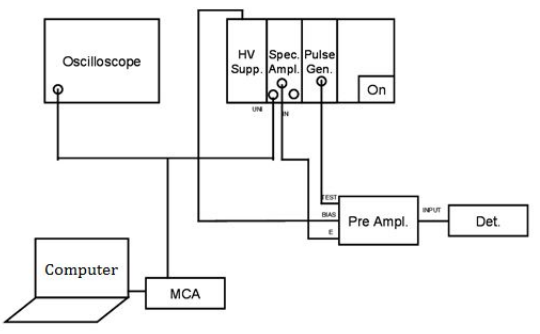
\includegraphics[width=.5\linewidth]{experimental_setup}
  \caption{Schema of the experimental setup}
  \label{fig:exp_setup}
\end{figure}
%%% Local Variables:
%%% mode: latex
%%% TeX-master: "prop_counter"
%%% End:
